\documentclass[12pt]{article}
\usepackage[top=1in, bottom=1in, left=1in, right=1in]{geometry}
%\usepackage[margin=1in]{geometry}
\usepackage[onehalfspacing]{setspace}
%\usepackage[doublespacing]{setspace}
\usepackage{amsmath, amssymb, amsthm}
\usepackage{enumerate, enumitem}
\usepackage{fancyhdr, graphicx, proof, comment, multicol}
\usepackage[none]{hyphenat} % This command prevents hyphenation of words
\binoppenalty=\maxdimen % This command and the next prevent in-line equation breaks
\relpenalty=\maxdimen
%    Good website with common symbols
% http://www.artofproblemsolving.com/wiki/index.php/LaTeX%3ASymbols
%    How to change enumeration using enumitem package
% http://tex.stackexchange.com/questions/129951/enumerate-tag-using-the-alphabet-instead-of-numbers
%    Quick post on headers
% http://timmurphy.org/2010/08/07/headers-and-footers-in-latex-using-fancyhdr/
%    Info on alignat
% http://tex.stackexchange.com/questions/229799/align-words-next-to-the-numbering
% http://tex.stackexchange.com/questions/43102/how-to-subtract-two-equations
%    Text align left-center-right
% http://tex.stackexchange.com/questions/55472/how-to-make-text-aligned-left-center-right-in-the-same-line
\usepackage{microtype} % Modifies spacing between letters and words
\usepackage{mathpazo} % Modifies font. Optional package.
\usepackage{mdframed} % Required for boxed problems.
\usepackage{parskip} % Left justifies new paragraphs.
\linespread{1.1} 


%figure support
\usepackage{import}
\usepackage{xifthen}
\pdfminorversion=7
\usepackage{pdfpages}
\usepackage{transparent}
\newcommand{\incfig}[1]{%
	\def\svgwidth{\columnwidth}
	\import{./figures/}{#1.pdf_tex}
}
\graphicspath{ {./figures/} }
\pdfsuppresswarningpagegroup=1

\newenvironment{problem}[1]
{\begin{mdframed}[linewidth=0.8pt]
        \textsc{Problem #1:}

}
    {\end{mdframed}}

\newenvironment{solution}
    {\textsc{Solution:}\\}
    {\newpage}% puts a new page after the solution
    
\newenvironment{statement}[1]
{\begin{mdframed}[linewidth=0.6pt]
        \textsc{Statement #1:}

}
    {\end{mdframed}}

%\newenvironment{prf}
 %   {\textsc{Proof:}\\}
 %   {\newpage}% puts a new page after the solution

\begin{document}
% This is the Header
% Make sure you update this information!!!!
\noindent
\textbf{CIS4367.01} \hfill \textbf{Brandon Thompson} \\
\normalsize Prof. Elibol \hfill Due Date: 2/19/20 \\

% This is where you name your homework
\begin{center}
\textbf{Homework 8}
\end{center}
	\begin{problem}{\#4.1}
		For the DAC model discussed In Section 4.3 , an alternative representation
		of the protection state is a directed graph. Each subject and each object
		in the protection state is represented by a node (a single node Is used for
		an entity that is both subject and object). A directed line from a subject
		to an object indicates an access right, and the label on the link defines
		the access right.
		\begin{enumerate}[label=\alph*]
			\item Draw a directed graph that corresponds to the access matrix
				of Figure 4.2a.
				%figure
			\item Draw a directed graph that corresponds to the access matrix
				of Figure 4.3.
				%figure
			\item Is there a one-to-one correspondence between the directed graph
				representation and the access matrix representation? Explain.
		\end{enumerate}
	\end{problem}
	\begin{figure}[ht!]
		\centering
		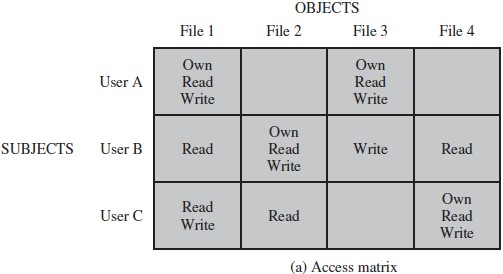
\includegraphics[width=0.8\textwidth]{fig4_2a}
	\end{figure}
	\begin{figure}[ht!]
		\centering
		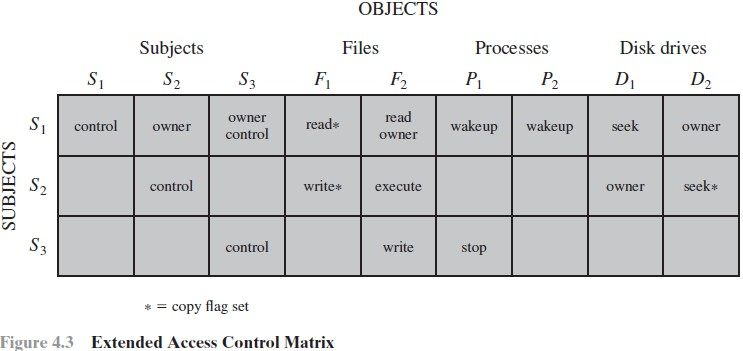
\includegraphics[width=0.8\textwidth]{fig4_3}
	\end{figure}
	\vspace{20em}
	\begin{solution}
		\begin{figure}[h!]
			\centering
			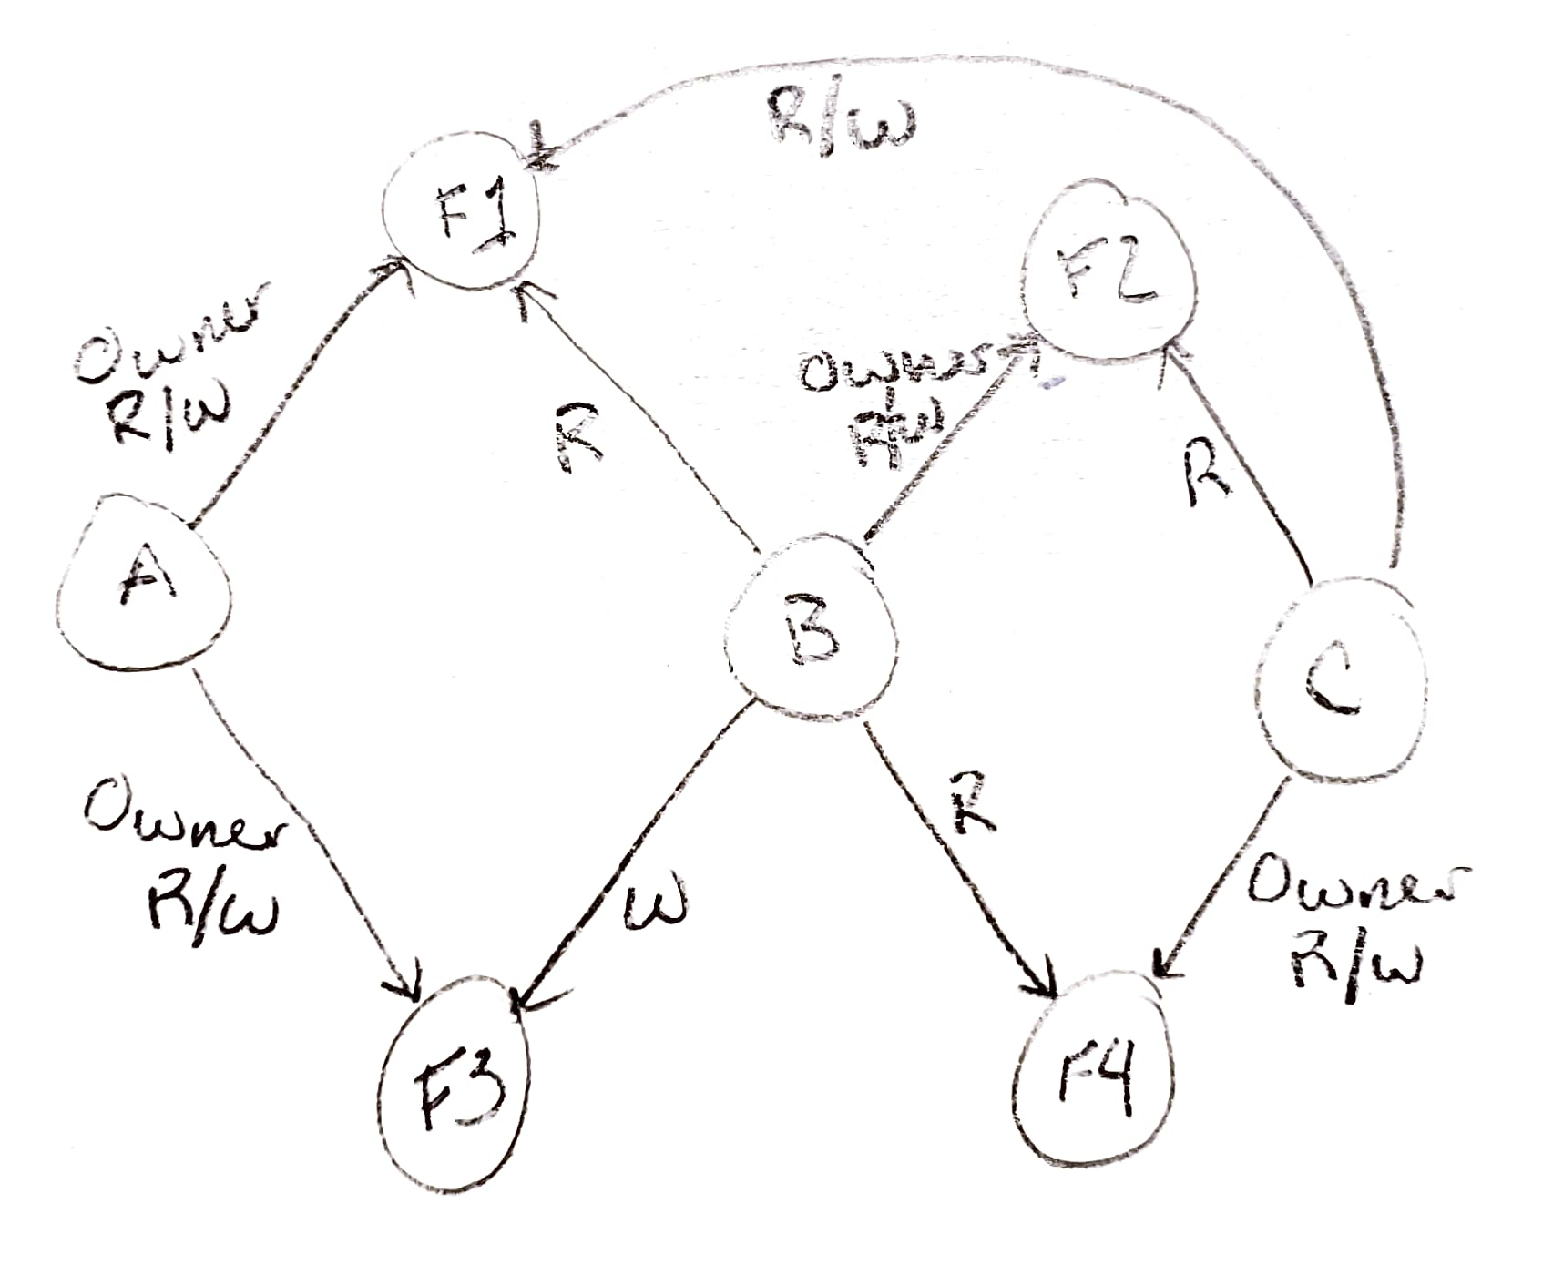
\includegraphics[width=0.6\textwidth]{ans4_1a}
			\caption{Answer for \textbf{a}.}
		\end{figure}
		\begin{figure}[ht!]
			\centering
			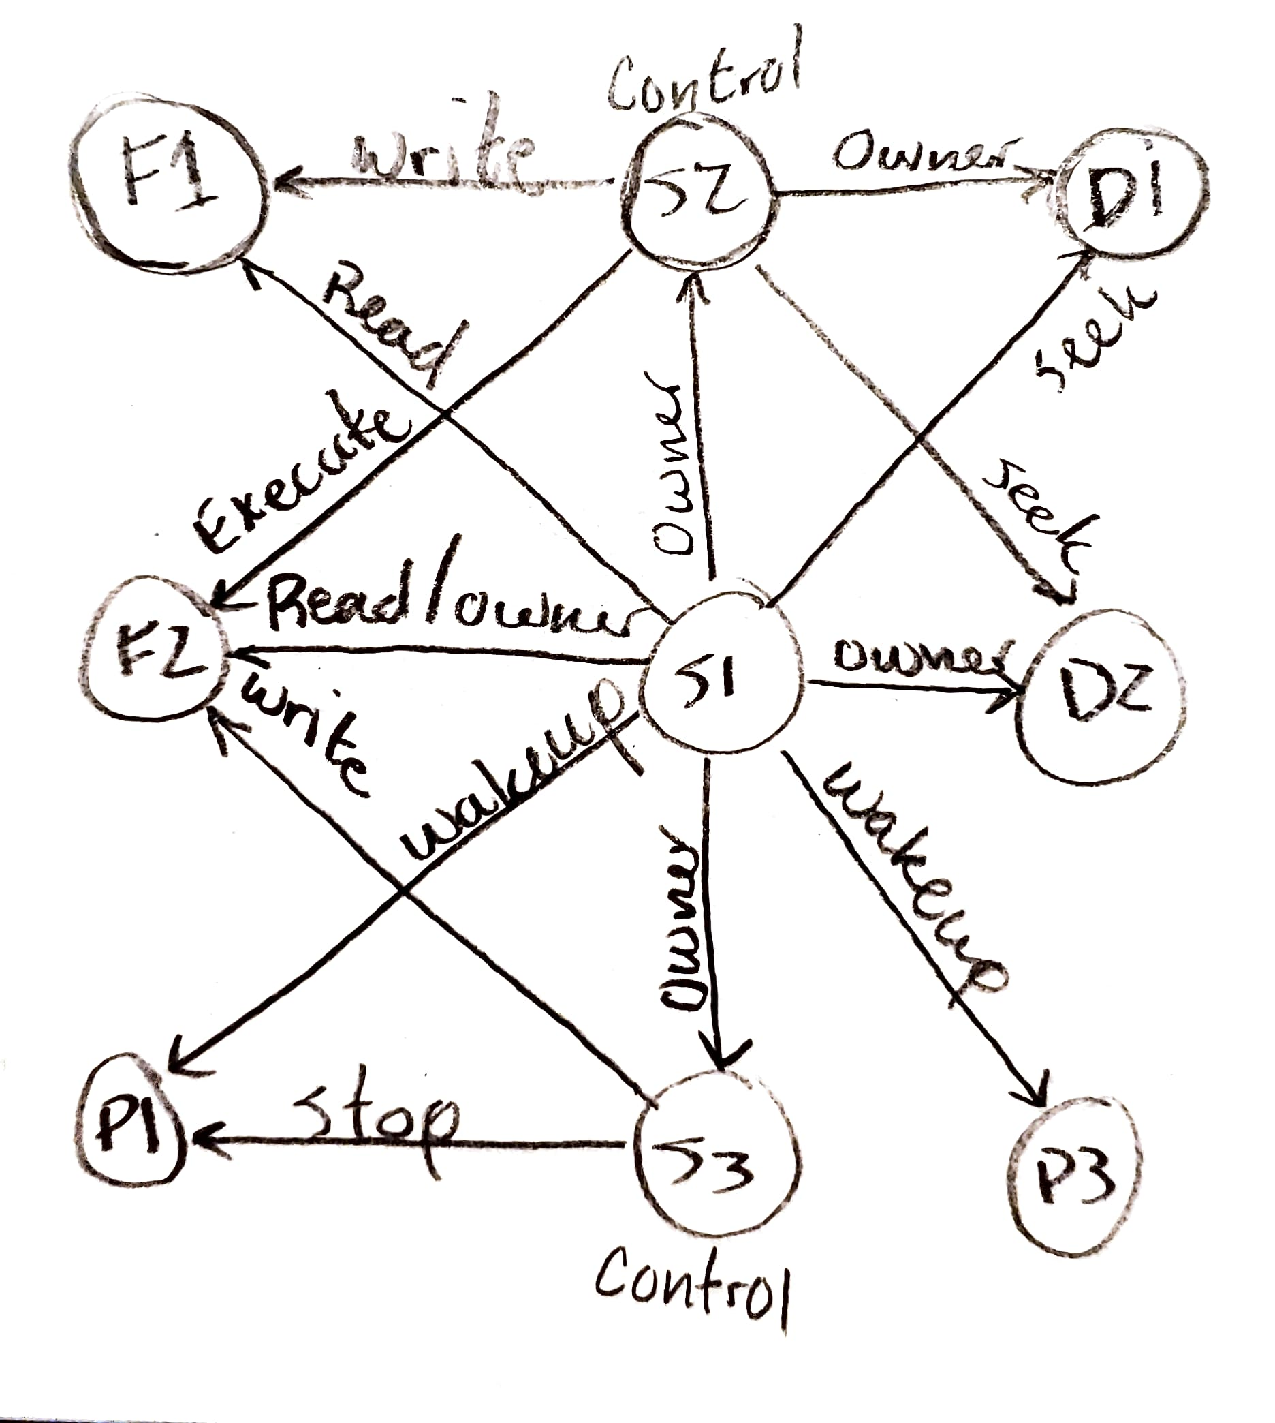
\includegraphics[width=0.6\textwidth]{ans4_1b}
			\caption{Answer for \textbf{b}.}
			\label{fig:ans4_1b}
		\end{figure}
		Yes, there is a one-to-one correspondence between the directed graph and the
		access representation.\\

		Since the access matrix passes all the respective edges from a user node to a file
		node when transposed to a directed graph. The users are one dimension of the matrix
		and the files another.

		In the directed graph, the user nodes are the top and the files are the bottom.
		Access is granted to users for a file so there is an edge from a user to a file.
	\end{solution}

	\begin{problem}{\#4.2}
		\begin{enumerate}[label=\alph*]
			\item Suggest a way of implementing protection domains using access control lists. 
			\item Suggest a way of implementing protection domains using capability tickets. 
		\end{enumerate}
		\textit{Hint: In both cases a level of indirection is required.}
	\end{problem}
	\begin{solution}
		\begin{itemize}[label=\alph*]
			\item The implementation of subject objects that are not associated with any user.
				\\
				The subject is a protection domain and it receives all of the privileges 
				of the access control list.
				\\
				Being on the subject is similar to being in the protection domain.
			\item Only processes holding a capability ticket to enter a protection
				domain are able to enter the domain.
		\end{itemize}	
	\end{solution}

	\begin{problem}{\#4.3}
		The VAXVMS operating system makes use of four processor access modes to
		facilitate the protection and sharing of system resources among processes.
		The access mode determines:
		\begin{itemize}
			\item \textbf{Instruction execution privileges:} What instructions
				the processor may execute.
			\item \textbf{Memory access privileges:} Which locations in virtual
				memory the current instruction may access
		\end{itemize}
		The four modes are as follows:
		\begin{itemize}
			\item \textbf{Kernel:} Executes the kernel of the VMS operating system,
				which includes memory management, interrupt handling, and
				I/O operations
			\item \textbf{Executive:} Executes many of the operating system service
				calls, including file and record (disk and tape)
				management routines
			\item \textbf{Supervisor:} Executes other operating system services,
				such as responses to user commands
			\item \textbf{User:} Executes user programs, plus utilities such as compilers,
				editors, linkers, and debuggers
		\end{itemize}
		A process executing in a less-privileged mode often needs to call a procedure that
		executes in a more-privileged mode; for example, a user program requires an
		operating system service. This call is achieved by using a change-mode (CHM)
		instruction, which causes an interrupt that transfers control to a routine at
		the new access mode. A return is made by executing the REI (return from exception
		or interrupt) instruction.
		\begin{enumerate}[label=\alph*]
			\item A number of operating systems have two modes, kernel and user.
				What are the advantages and disadvantages of providing four
				modes instead of two?
			\item Can you make a case for even more than four modes?
		\end{itemize}
	\end{problem}
	\begin{solution}
		\begin{itemize}[label=\alph*]
			\item If the system has four modes then it is better able to control access
				to the system. The cost of having four modes is the system is much
				more complex.
			\item If a system needed more flexibility to manage users (maybe a mode for
				every type of user) then you would need more modes. This seems
				unnecessarily complex though.
		\end{itemize}
	\end{solution}

	\begin{problem}{\#4.4}
		The VMS scheme discussed in the preceding problem is often referred to as a ring
		protection structure, as illustrated in Figure 4.15. Indeed, the simple kernel/user
		scheme is a two-ring structure. A disadvantage of a ring-structured access control
		system is that it violates the principal of least privilege. For example if we wish
		to have an object accessible in ring $X$ but not in ring $Y$, this requires that
		$X < Y$. Under this arrangement all objects accessible in ring $X$ are also accessible
		in ring $Y$.
		\begin{enumerate}[label=\alph*]
			\item Explain in more detail what the problem is and why least privilege is
				violated.
		\end{enumerate}
	\end{problem}
	\begin{solution}
		Least privilege is violated because users should have as little access possible and
		still maintain functionality. If a user is a part of ring $X$ and needs to keep
		something from ring  $Y$ then x would be able to access everything in  $Y$. But
		because  $X$ does not need everything in  $Y$ least privilege is violated.
	\end{solution}

	\begin{problem}{\#4.5}
		UNIX treats file directories in the same fashion as files; that is, both are defined
		by the same type of data structure, called an inode. As with files, directories 
		include a nine-bit protection string. If care is not take, this can create access
		control problems. For example, consider a file with protection mode 644 (octal)
		contained in a directory with protection mode 730. How might the file be compromised
		in this case?
	\end{problem}
	\begin{solution}
		File protection mode 644 gives the owner read and write privileges, groups get read access
		and  others get read access. Directory protection code 730 gives owner read, write,
		and execute, Group users get write and execute. Others get nothing.\\

		The permissions given to the file are no use because the directory overrides the
		file permissions. Others cannot read the file and members of the group can change or delete
		the file.
	\end{solution}

	\begin{problem}{\#4.6}
		In the traditional UNIX file access model, which we described in Section 4.4, UNIX
		systems provide a default setting for newly created files and directories, which
		the owner may later change. The default is typically full access for the owner 
		combined with one of the following: no access for group and other, read/execute
		access for group and none for other, or read/execute for both group and other.
		Briefly discuss the advantages and disadvantages of each of these cases, including
		an example of a type of organization where each would be appropriate.
	\end{problem}
	\begin{solution}
		\begin{enumerate}
			\item Default full access rights for owner and none for group and others.\\
				Advantages:
				\begin{itemize}
					\item Files are secure from tampering and eavesdropping.
				\end{itemize}
				Disadvantages:
				\begin{itemize}
					\item Access must be given explicitly to each user.
				\end{itemize}
				Example: This is the most common default permission because it
				offers the best security for when the user wants to keep things confidential,
				like Government agencies or businesses working with proprietary information.
			\item Default full access rights for owner, read and execute for group, none for others.\\
				Advantages:
				\begin{itemize}
					\item Files protected from unauthorized users.
					\item Files can be shared with other users.
				\end{itemize}
				Disadvantages:
				\begin{itemize}
					\item Compromised account could damage company by
						getting access to confidential files.
				\end{itemize}
				Example: Used for teams working on a project together on a server.
			\item Default full access for owner, read and execute for group and others.\\
				Advantages:
				\begin{itemize}
					\item Improved work efficiency because everyone can access everything.
					\item Information is available to all users.
				\end{itemize}
				Disadvantages:
				\begin{itemize}
					\item Everyone has access so confidential data is not secure.
				\end{itemize}
				Example: Research facility or small businesses can benefit from this structure.
		\end{enumerate}
	\end{solution}

	\begin{problem}{\#4.7}
		Consider user accounts on a system with a Web server configured to provide access
		to user Web areas. In general, this uses a standard directory name, such as
		`public\_html,' in a user's home directory. This acts as their user Web area if it
		exists. However, to allow the Web server to access the pages in this directory, it
		must have at least search (execute) access to the user's home directory,
		read/execute access to the Web directory, and read access to any Web pages in it.
		Consider the interaction of this requirement with the cases you discussed for the
		preceding problem. What consequences does this requirement have? Note that a Web
		server typically executes as a special user, and in a group that is not shared
		with most users on the system. Are there some circumstances when running such a
		Web service is simply not appropriate? Explain.
	\end{problem}
	\begin{solution}
		If the users files are of a sensitive nature, the risk of accidental leakage because
		of incorrect permissions may stop you from using a web server.\\
		Failure to set correct permissions for every new directory could not grant access
		to the directory through the web server.
	\end{solution}

	\begin{problem}{\#4.9}
		The NIST RBAC standard defines a limited role hierarchy as one in which a role
		may have one or more immediate ascendants but is restricted to a single immediate
		descendant. What inheritance relationships in Figure 4.10 are prohibited by the
		NIST standard for a limited role hierarchy?
	\end{problem}
	\begin{solution}
		The Access Control Mechanism would not follow the guidelines of limited
		role hierarchy because the access control mechanism pulls from many
		different attributes and give one of two possible answers.
	\end{solution}

	\begin{problem}{\#4.11}
		In the example of Section 4.8, use the notation \textit{Role(x).Position} to denote
		to position associated with role $x$ and \textit{Role(x).Function} to denote
		to function associated with role $x$.
		\begin{enumerate}[label=\alph*]
			\item We define the role hierarchy for this example as one in which
				one role is superior to another if its position is superior
				and their functions are identical. Express this relationship
				formally.
			\item An alternative role hierarchy is one in which a role is superior
				to another if its function is superior, regardless of position.
				Express this relationship formally.
		\end{enumerate}
	\end{problem}
	\begin{solution}
		\begin{enumerate}[label=\alph*]
			\item \ \ 
				\begin{center}
					\textit{Role(x)} $>$ \textit{Role(y)}$\implies$ \textit{Role(x).Position} $>$
					\textit{Role(y).position}  $\wedge$ \\
					\textit{Role(x).Function}  $=$ \textit{Role(y).Function}
				\end{center}
				Role $x$ is greater than role $y$ if the position of $x$ is greater than
				the position of $y$ and the function of both are equal.
			\item \ \
				\begin{center}
					\textit{Role(x)} $>$ \textit{Role(y)}  $\implies$ \textit{Role(x).Function} 
					$>$ \textit{Role(y).Function}
				\end{center}
				Role $x$ is greater than role $y$ if the function of $x$ is greater
				than the function of $y$. Position does not matter.
		
		\end{enumerate}
	\end{solution}
\end{document}
